\documentclass[a4paper, 14pt]{extarticle}

% Поля
%--------------------------------------
\usepackage{geometry}
\geometry{a4paper,tmargin=2cm,bmargin=2cm,lmargin=3cm,rmargin=1cm}
%--------------------------------------


%Russian-specific packages
%--------------------------------------
\usepackage[T2A]{fontenc}
\usepackage[utf8]{inputenc} 
\usepackage[english, main=russian]{babel}
%--------------------------------------

\usepackage{textcomp}

% Красная строка
%--------------------------------------
\usepackage{indentfirst}               
%--------------------------------------             


%Graphics
%--------------------------------------
\usepackage{graphicx}
\graphicspath{ {./images/} }
\usepackage{wrapfig}
%--------------------------------------

% Полуторный интервал
%--------------------------------------
\linespread{1.3}                    
%--------------------------------------

%Выравнивание и переносы
%--------------------------------------
% Избавляемся от переполнений
\sloppy
% Запрещаем разрыв страницы после первой строки абзаца
\clubpenalty=10000
% Запрещаем разрыв страницы после последней строки абзаца
\widowpenalty=10000
%--------------------------------------

%Списки
\usepackage{enumitem}

%Подписи
\usepackage{caption} 

%Гиперссылки
\usepackage{hyperref}

\hypersetup {
	unicode=true
}

%Рисунки
%--------------------------------------
\DeclareCaptionLabelSeparator*{emdash}{~--- }
\captionsetup[figure]{labelsep=emdash,font=onehalfspacing,position=bottom}
%--------------------------------------

\usepackage{tempora}

%Листинги
%--------------------------------------
\usepackage{listings}
\lstset{
  basicstyle=\ttfamily\footnotesize, 
  %basicstyle=\footnotesize\AnkaCoder,        % the size of the fonts that are used for the code
  breakatwhitespace=false,         % sets if automatic breaks shoulbd only happen at whitespace
  breaklines=true,                 % sets automatic line breaking
  captionpos=t,                    % sets the caption-position to bottom
  inputencoding=utf8,
  frame=single,                    % adds a frame around the code
  keepspaces=true,                 % keeps spaces in text, useful for keeping indentation of code (possibly needs columns=flexible)
  keywordstyle=\bf,       % keyword style
  numbers=left,                    % where to put the line-numbers; possible values are (none, left, right)
  numbersep=5pt,                   % how far the line-numbers are from the code
  xleftmargin=25pt,
  xrightmargin=25pt,
  showspaces=false,                % show spaces everywhere adding particular underscores; it overrides 'showstringspaces'
  showstringspaces=false,          % underline spaces within strings only
  showtabs=false,                  % show tabs within strings adding particular underscores
  stepnumber=1,                    % the step between two line-numbers. If it's 1, each line will be numbered
  tabsize=2,                       % sets default tabsize to 8 spaces
  title=\lstname                   % show the filename of files included with \lstinputlisting; also try caption instead of title
}
%--------------------------------------

%%% Математические пакеты %%%
%--------------------------------------
\usepackage{amsthm,amsfonts,amsmath,amssymb,amscd}  % Математические дополнения от AMS
\usepackage{mathtools}                              % Добавляет окружение multlined
\usepackage[perpage]{footmisc}
%--------------------------------------

%--------------------------------------
%			НАЧАЛО ДОКУМЕНТА
%--------------------------------------

\begin{document}

%--------------------------------------
%			ТИТУЛЬНЫЙ ЛИСТ
%--------------------------------------
\begin{titlepage}
\thispagestyle{empty}
\newpage


%Шапка титульного листа
%--------------------------------------
\vspace*{-60pt}
\hspace{-65pt}
\begin{minipage}{0.3\textwidth}
\hspace*{-20pt}\centering

\includegraphics[width=\textwidth]{emblem}
\end{minipage}
\begin{minipage}{0.67\textwidth}\small \textbf{
\vspace*{-0.7ex}
\hspace*{-6pt}\centerline{Министерство науки и высшего образования Российской Федерации}
\vspace*{-0.7ex}
\centerline{Федеральное государственное бюджетное образовательное учреждение }
\vspace*{-0.7ex}
\centerline{высшего образования}
\vspace*{-0.7ex}
\centerline{<<Московский государственный технический университет}
\vspace*{-0.7ex}
\centerline{имени Н.Э. Баумана}
\vspace*{-0.7ex}
\centerline{(национальный исследовательский университет)>>}
\vspace*{-0.7ex}
\centerline{(МГТУ им. Н.Э. Баумана)}}
\end{minipage}
%--------------------------------------

%Полосы
%--------------------------------------
\vspace{-25pt}
\hspace{-35pt}\rule{\textwidth}{2.3pt}

\vspace*{-20.3pt}
\hspace{-35pt}\rule{\textwidth}{0.4pt}
%--------------------------------------

\vspace{1.5ex}
\hspace{-35pt} \noindent \small ФАКУЛЬТЕТ\hspace{80pt} <<Информатика и системы управления>>

\vspace*{-16pt}
\hspace{47pt}\rule{0.83\textwidth}{0.4pt}

\vspace{0.5ex}
\hspace{-35pt} \noindent \small КАФЕДРА\hspace{50pt} <<Теоретическая информатика и компьютерные технологии>>

\vspace*{-16pt}
\hspace{30pt}\rule{0.866\textwidth}{0.4pt}
  
\vspace{11em}

\begin{center}
\Large {\bf Лабораторная работа № 10} \\ 
\large {\bf по курсу <<Языки и методы программирования>>} \\
\large <<Реализация итераторов на языке C++>> \\
\Large Вариант 4
\end{center}\normalsize

\vspace{8em}


\begin{flushright}
  {Студент группы ИУ9-21Б Шиятов Н. \hspace*{15pt}\\ 
  \vspace{2ex}
  Преподаватель Посевин Д. П.\hspace*{15pt}}
\end{flushright}

\bigskip

\vfill
 

\begin{center}
\textsl{Москва 2023}
\end{center}
\end{titlepage}
%--------------------------------------
%		КОНЕЦ ТИТУЛЬНОГО ЛИСТА
%--------------------------------------

\renewcommand{\ttdefault}{pcr}

\setlength{\tabcolsep}{3pt}
\newpage
\setcounter{page}{2}

\section{Задание}\label{Sect::task}

Требуется составить контейнерный класс и итератор для перебора содержимого объектов этого
класса.

Последовательность простых дробей с
однонаправленным итератором по суммам
соседних дробей. Обращение к элементам
последовательности должно осуществлятся с
помощью перегруженной операции «[ ]».
Изменение суммы двух соседних дробей
посредством итератора должно отражаться на
величине первой дроби.

\section{Результаты}\label{Sect::res}

Исходный код программы представлен в листингах~\ref{lst:fraction}--~\ref{lst:main}.

Результат запуска представлен на рисунке~\ref{fig:output}.

\begin{figure}[!htb]
\begin{lstlisting}[language=Java,caption={Код класса Fraction},label={lst:fraction}]
#include <iostream>
#include <utility>
#include <vector>

using namespace std;

class Fraction {
private:
    int numerator, denominator;

    void simplify() {
        int t = GCD(numerator, denominator);
        this->numerator = numerator / t;
        this->denominator = denominator / t;
    };
public:
    Fraction() : numerator(1), denominator(1) {};

    Fraction(int numerator, int denominator) : numerator(numerator), denominator(denominator) {
        simplify();
    }

    static int GCD(int a, int b) {
        return b ? GCD(b, a % b) : a;
    }

    static int LCM(int a, int b) {
        return a / GCD(a, b) * b;
    }

    friend Fraction sum(Fraction a, Fraction b) {
        int numerator1 = a.numerator, denominator1 = a.denominator;
        int numerator2 = b.numerator, denominator2 = b.denominator;
        int lcm = LCM(denominator1, denominator2);
        numerator1 *= lcm / denominator1;
        numerator2 *= lcm / denominator2;
        int x = numerator1 + numerator2;
        return {x, lcm};
    }

    friend Fraction operator+(const Fraction &a, const Fraction &b) {
        return sum(a, b);
    }

    friend ostream &operator<<(ostream &output, const Fraction &frac) {
        output << frac.numerator << "/" << frac.denominator;
        return output;
    }

    friend istream &operator>>(istream &in, Fraction &frac) {
        in >> frac.numerator >> frac.denominator;
        frac.simplify();
        return in;
    }
};
\end{lstlisting}
\end{figure}

\begin{figure}[!htb]
\begin{lstlisting}[language=Java,caption={Код класса FractionSequence},label={lst:sequence}]
class FractionSequence {
private:
    vector<Fraction> sequence;

    class Iterator {
        vector<Fraction>::iterator cur;
    public:
        Iterator(vector<Fraction>::iterator first) : cur(first) {}

        Iterator operator++(int) {
            Iterator temp = *this;
            cur++;
            return temp;
        }

        bool operator!=(const Iterator &it) {
            return cur != it.cur;
        }

        bool operator==(const Iterator &it) {
            return cur == it.cur;
        }

        Iterator operator+=(Fraction x) {
            *cur = *cur + x;
            return *this;
        }

        Fraction operator*() {
            return *cur + *(cur + 1);
        }
    };

public:
    explicit FractionSequence(vector<Fraction> s) : sequence(std::move(s)) {}

    void add(int numerator, int denominator) {
        sequence.emplace_back(numerator, denominator);
    }

    Fraction &operator[](int index) {
        return sequence[index];
    }

    Iterator begin() {
        return {sequence.begin()};
    }

    Iterator end() {
        return {sequence.end() - 1};
    }
};
\end{lstlisting}
\end{figure}

\begin{figure}[!htb]
\begin{lstlisting}[language=Java,caption={Код функции main},label={lst:main}]
#include "FractionSequence.cpp"
#include <iostream>

using namespace std;

int main() {
    FractionSequence sequence({
        Fraction(1, 2),
        Fraction(1, 3),
    });
    sequence.add(3, 4);

    for (int i = 0; i < 3; i++){
        cout << sequence[i] << "  ";
    }
    cout << endl;


    for (auto it = sequence.begin(); it != sequence.end(); it++) {
        cout << *it << "  ";
    }
    cout << endl;


    for (auto it = sequence.begin(); it != sequence.end(); it++){
        it += {1, 3};
        cout << *it << "  ";
    }
    cout << endl;


    for (int i = 0; i < 3; i++) {
        cout << sequence[i] << "  ";
    }

    return 0;
}
\end{lstlisting}
\end{figure}


\begin{figure}[!htb]
	\centering
	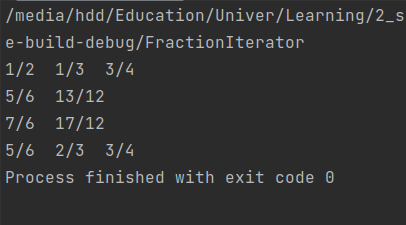
\includegraphics[width=0.8\textwidth]{output.png}
\caption{Результат работы}
\label{fig:output}
\end{figure}

\end{document}
